\chapter{Électronique} \label{electronique}
\section{Microcontrôleur}

\subsection{Introduction}

\subsection{Microprocesseur (\textit{µP})}
Un \textbf{microprocesseur} (\textit{µP}) est une 
\textbf{unité centrale de traitement} (\textbf{CPU}\footnote{Glossaire : \gls{cpu}}) qui exécute des 
instructions, mais qui \textbf{ne contient ni mémoire RAM, ni mémoire ROM, ni 
entrées/sorties intégrées}. Il est conçu pour des systèmes où ces composants, 
tels que la \textit{RAM}, la \textit{ROM}, et les \textit{interfaces}, sont 
ajoutés séparément sur une carte mère. Le \textit{microprocesseur} est 
principalement utilisé dans les \textbf{ordinateurs}, \textbf{serveurs}, et 
\textbf{systèmes embarqués avancés}, comme les processeurs Intel, AMD, ou Apple 
Silicon.\par

\subsection{Microcontrôleur (\textit{MCU})}
Un \textbf{microcontrôleur} (\textit{MCU}) est un \textbf{circuit intégré complet} 
qui inclut non seulement un \textbf{microprocesseur}, mais aussi de la 
\textbf{mémoire RAM}, de la \textbf{mémoire ROM (Flash)} et des 
\textbf{périphériques d'entrées/sorties} sur une seule puce. Cela lui confère un 
\textbf{plus haut degré d'intégration} par rapport à un microprocesseur. Il est 
également appelé un \textbf{Système sur une Puce} (\textbf{SoC}, 
\textit{System On a Chip}). Il est conçu pour exécuter des 
\textbf{tâches spécifiques} à un \textbf{coût réduit} et avec une 
\textbf{consommation d'énergie optimisée}. On le retrouve dans des 
\textbf{systèmes embarqués}, notamment dans des 
\textbf{appareils électroménagers}, des \textbf{voitures}, des 
\textbf{jouets électroniques}, et des \textbf{objets connectés}, comme les 
dispositifs basés sur \textit{Arduino}, \textit{STM32}, \textit{PIC}, et 
\textit{ESP32}.\par

\section{Le microcontrôleur ESP32}

Le microcontrôleur utilisé dans la mineure \textbf{Instrumentation} est 
l'\textbf{ESP32}, fabriqué par \textbf{Espressif Systems} (\textit{Chine}).

\subsection{Caractéristiques principales de l'ESP32}
Le \textbf{processeur} de l'ESP32 est un \textit{Dual-Core Xtensa LX6} qui peut 
fonctionner jusqu'à \SI{240}{\mega\hertz}, conçu par \textbf{Tensilica}. Il
dispose également d' \textbf{instructions DSP} (\textit{Digital Signal Processing}) 
intégrées, permettant le \textbf{traitement de signaux complexes}. En termes de 
\textbf{connectivité}, l'ESP32 supporte le \textbf{Wi-Fi}, le \textbf{Bluetooth}, 
ainsi que le \textbf{Bluetooth Low Energy (BLE)}. Il dispose également de 
\textbf{modes basse consommation}, ce qui est crucial pour les applications à 
faible consommation énergétique. Parmi les \textbf{interfaces de périphériques} 
disponibles, on trouve :
\begin{itemize}
    \item \textbf{CAN} (Convertisseur \textbf{DAC})
    \item \textbf{CNA} (Convertisseur \textbf{ADC})
    \item \textbf{Capteur de toucher}
    \item \textbf{SPI}, \textbf{I2C}, \textbf{I2S}, \textbf{CAN}, \textbf{UART}, \textbf{PWM}
\end{itemize}

\begin{figure}[!ht]
    \centering
    \includegraphics[width=0.9\textwidth]{esp32-block}
    \caption{Microcontrôleur ESP32}
    \label{fig:esp32}
\end{figure}

\subsection{Carte de développement ESP32-WROVER-B}
Le \textbf{microcontrôleur ESP32} est intégré dans une
 \textbf{carte de développement} basée sur le module \textbf{ESP32-WROVER-B}, 
 fabriqué par \textbf{uPesy} (\textit{France}), sous la référence 
 \textbf{ESP32 Wrover DevKit v2.1}. Cette carte présente plusieurs 
 \textbf{avantages} :
\begin{itemize}
    \item \textbf{Brochage des principales entrées/sorties}, facilitant ainsi son utilisation pour le prototypage.
    \item \textbf{Alimentation et connexion USB-C} intégrées pour un usage simplifié.
    \item \textbf{Mémoire supplémentaire} pour des applications plus complexes.
    \item \textbf{Compatibilité breadboard}, idéale pour la réalisation de \textbf{prototypes}.
\end{itemize}


\section{Amplificateur opérationnel}\label{electronique:opamp}

Un \textbf{amplificateur opérationnel} est un dispositif électronique permettant 
d'amplifier une différence de tension. Il est également appelé \textit{Ampli OP}, 
\textit{AOP} ou \textit{ALI} (\textbf{Amplificateur Linéaire Intégré}). Il 
possède deux entrées, notées \(V_+\) et \(V_-\), ainsi qu'une sortie 
\(V_s\). La sortie de l'amplificateur opérationnel correspond au produit de 
la différence de tension entre les deux entrées, multiplié par un facteur, 
souvent très élevé.

C'est un \textbf{circuit actif}, ce qui signifie qu'il a besoin d'une 
alimentation externe pour fonctionner. Il nécessite à la fois une alimentation 
positive (\(V_{CC+}\)) et une alimentation négative (\(V_{CC-}\)). Dans 
certains cas, l'alimentation négative peut être fournie par la masse 
(\(V_{CC-} = \text{masse}\)).


\begin{minipage}{0.49\textwidth}
    \begin{figure}[H]
        \centering
        \includegraphics[width=0.9\textwidth]{opamp}
        \caption{Amplificateur opérationnel}
        \label{fig:opamp}
    \end{figure}
\end{minipage}
\begin{minipage}{0.5\textwidth}
    \begin{figure}[H]
        \centering
        \includegraphics[width=0.3\textwidth]{MCP6271}
        \caption{Amplificateur opérationnel MCP6271}
        \label{fig:opamp-symbol}
    \end{figure}
\end{minipage}

L'entrée \(V_+\) est aussi appelée \textbf{entrée non inverseuse} (notée 
\(+\) sur le schéma), tandis que l'entrée \(V_-\) est appelée 
\textbf{entrée inverseuse} (notée \(-\) sur le schéma). L'alimentation 
positive \(V_{CC+}\) est parfois aussi désignée sous les appellations
\(V_{DD}\), \(V_{CC}\) ou \(V_{S+}\). De même, l'alimentation négative 
\(V_{CC-}\) peut être nommée \(V_{SS}\), \(V_{EE}\), \(V_{S-}\) ou 
encore \textbf{GND} si elle est connectée à la masse.

\section{Généralités sur les AOP}

L'alimentation électrique d'un \textbf{amplificateur opérationnel} (\textbf{AOP}
) peut être de deux types :
\begin{itemize}
    \item Une \textbf{alimentation simple} (\textit{single supply}), purement 
            positive, par exemple \SI{0}{\volt} / \SI{+12}{\volt}.
    \item Une \textbf{alimentation symétrique} (\textit{dual supply}), où l'on 
    dispose d'une tension négative et positive, par exemple \SI{-15}{\volt} / 
    \SI{+15}{\volt}.
\end{itemize}

Certains AOP fonctionnent exclusivement avec une alimentation symétrique, 
d'autres uniquement avec une alimentation simple, et certains peuvent accepter 
les deux modes (\textit{cf. datasheet du composant}). Il est important de noter 
que l'alimentation conditionne directement le niveau de tension en sortie : un 
AOP alimenté en \SI{-12}{\volt} / \SI{+12}{\volt} ne pourra délivrer qu'une 
tension de sortie comprise entre \SI{-12}{\volt} et \SI{+12}{\volt}.

Un amplificateur opérationnel ne s'utilise quasiment jamais seul. En pratique, 
il est accompagné de composants électroniques additionnels tels que des 
\textbf{résistances}, des \textbf{condensateurs} et des \textbf{inductances}. 
Ces composants permettent d'utiliser l'AOP dans diverses applications :
\begin{itemize}
    \item \textbf{Calculs mathématiques analogiques} : addition, soustraction, 
    inversion, intégration, dérivation, etc. Ces fonctions sont utilisées 
    notamment pour le \textbf{pilotage et la régulation de moteurs électriques}.
    \item \textbf{Filtrage de signaux analogiques} : réalisation de filtres 
    passe-bas, passe-haut, passe-bande, ou encore de filtres de rejet de bande. 
    Ces filtres sont exploités dans des applications telles que le 
    \textbf{filtrage audio}, le \textbf{mixage audio} ou encore l'atténuation de 
    \textbf{bruits électroniques}.
    \item \textbf{Amplification de tensions et de courants} : un AOP peut être 
    utilisé pour amplifier un signal avec adaptation d'impédance, ce qui est 
    essentiel en \textbf{pré-amplification}, en \textbf{amplification} 
    proprement dite, ainsi que pour la 
    \textbf{régulation de tension et de courant}.
\end{itemize}

En interne un AOP est en fait un assemblage de plusieurs transistors, resistances et condensateurs. 
Il est donc possible de le modéliser par un schéma équivalent plus simple, 
appelé \textbf{schéma de représentation équivalent}.
\begin{figure}[H]
    \centering
    \includegraphics[width=0.9\textwidth]{LM741}
    \caption{
        Schéma équivalent d'un amplificateur opérationnel LM741
    }
    \label{fig:opamp-equivalent}
\end{figure}

Dans le cas d'un \textbf{amplificateur opérationnel r\'eel}, on note la relation entrée
la sortie \(V_S\) et les tensions \(V_+\) et \(V_-\) :
\[
    V_S=G_{diff}\cdot\left(V^{+}-V^{-}\right)+G_{mc}\cdot\frac{V^{+}+V^{-}}{2}
\]

O\`u \(G_{diff}\) est le gain différentiel et \(G_{mc}\) le gain en mode commun.
Le gain en mode commun est souvent tr\`es faible, de l'ordre de \SI{100}{\micro\volt\per\volt}.
Le gain différentiel est tr\`es élevé, de l'ordre de \SI{100000}{\volt\per\volt}, 
on voit très vite que le moindre écart différentiel au niveau des entrées va 
représenter une grande tension en sortie..
Ainsi l'on peut approximer un \textbf{amplificateur opérationnel idéal} par la relation :

\begin{align*}
    V_S&=G_{diff}\cdot\left(V^{+}-V^{-}\right)\\
    V_S&=G_{diff}\cdot\epsilon
\end{align*}

Ce qui donne la vue interne simplifiée d'un AOP :\\
\begin{minipage}{0.79\textwidth}
    \begin{figure}[H]
        \centering
        \includegraphics[width=0.9\textwidth]{opamp2}
        \caption{Amplificateur opérationnel idéal}
        \label{fig:opamp-ideal}
    \end{figure}
\end{minipage}
\begin{minipage}{0.2\textwidth}
    \[
        V_{S}=G_{diff}\cdot\epsilon
    \]
\end{minipage}

\begin{example}.\\
    Si \(V^+=\SI{2345}{\volt}\) et \(V^-=\SI{2320}{\volt}\), alors \(\epsilon=\SI{25}{\milli\volt}\) et 
    \(V_S=G_{diff}\cdot\SI{25}{\milli\volt} = \SI{2500}{\volt}\).\\
    L'ampli Op ne sera bien évidemment pas capable de sortir une telle tension.
    La tension de sortie sera limitée à la tension d'alimentation positive ou
    négative suivant le cas.
\end{example}

\subsection{Régime linéaire et régime saturé}

L'amplificateur opérationnel peut adopter trois comportements distincts :

\begin{itemize}
    \item Si \( V_S < V_{CC-} \), l'AOP est en \textbf{saturation négative}, et la tension de sortie est bloquée à \( V_{CC-} \).
    \item Si \( V_S > V_{CC+} \), l'AOP est en \textbf{saturation positive}, et la tension de sortie est bloquée à \( V_{CC+} \).
    \item Si \( V_{CC-} < V_S < V_{CC+} \), l'AOP fonctionne en \textbf{régime linéaire}, et la relation suivante est valide :
    \[
    V_S = G_{\text{diff}} \times (V_+ - V_-)
    \]
\end{itemize}

En résumé, un amplificateur opérationnel peut fonctionner selon deux régimes principaux :

\begin{enumerate}
    \item En \textbf{régime linéaire}, où la tension de sortie suit l'équation :
    \[
    V_S = A \times (V_+ - V_-)
    \]
    \item En \textbf{régime saturé}, où la tension de sortie est contrainte à une valeur maximale ou minimale, correspondant aux tensions d'alimentation de l'AOP.
\end{enumerate}

\begin{figure}[!ht]
    \resizebox{\linewidth}{!}{%
    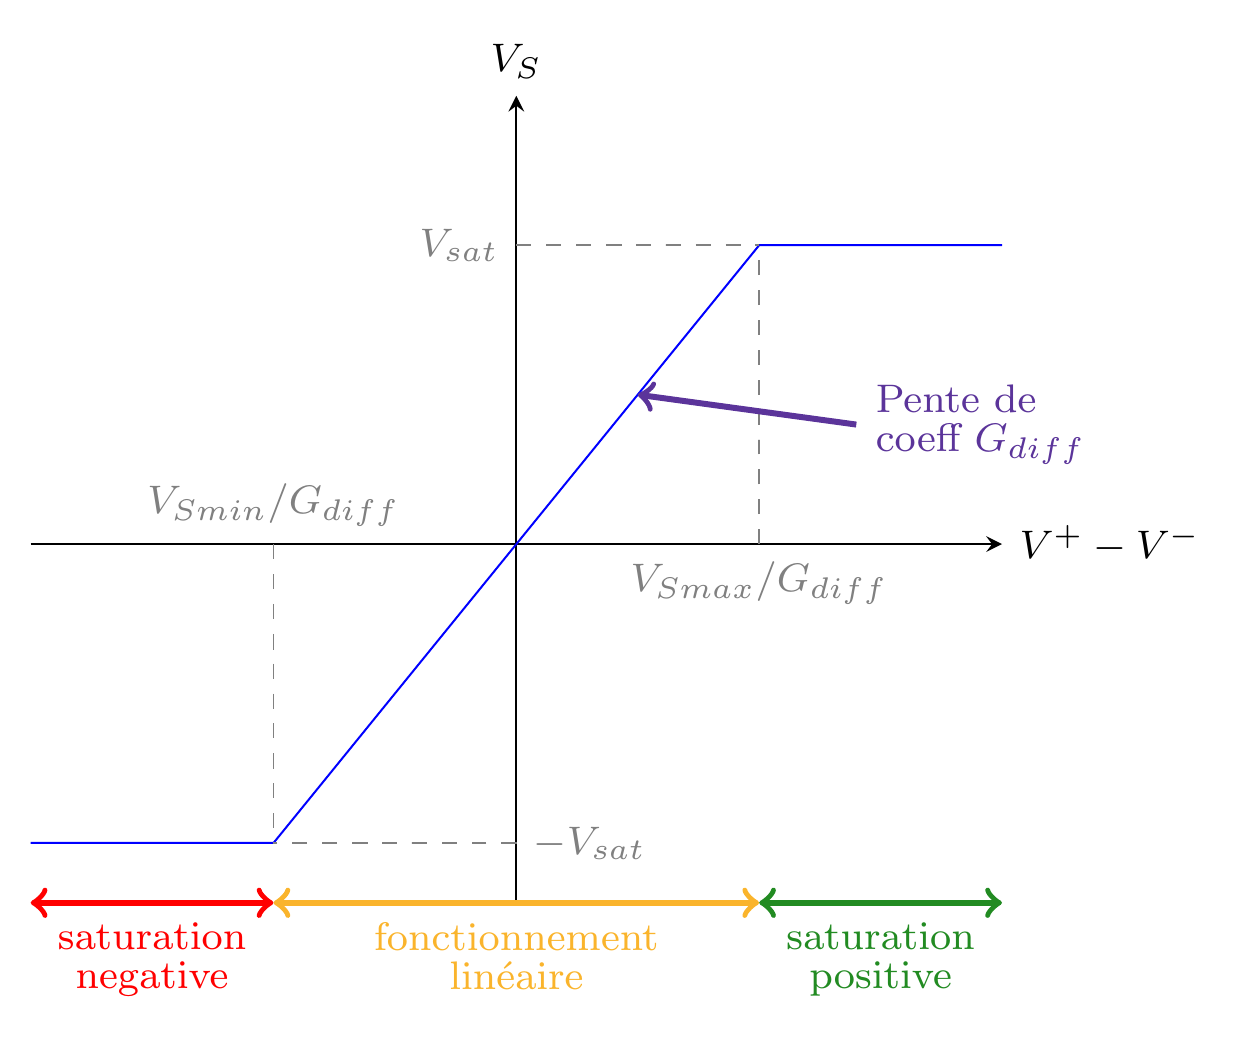
\begin{tikzpicture}[scale=1.8]
        \tikzstyle{every node}=[font=\fontsize{8}{8}\selectfont]
        \begin{axis}[
            axis y line=center,
            axis x line=middle, 
            ticks=none,
            xmin = -2,
            xmax = 2,
            ymin = -1.2,
            ymax = 1.5, 
            ylabel = \(V_S\),
            xlabel = \(V^+-V^-\),
            every axis x label/.style={
                at={(ticklabel* cs:1)},
                anchor=west,
            },
            every axis y label/.style={
                at={(ticklabel* cs:1)},
                anchor=south,
            },
            clip=false,
        ]
        \addplot+[mark=none,] coordinates
        {(-2,-1) (-1,-1) (1,1) (2,1)};
        \addplot[dashed, samples=50, smooth,domain=0:6,gray] coordinates {(1,0)(1,1)}node[below,pos=0] {\(V_{Smax}/G_{diff}\)};
        \addplot[dashed, samples=50, smooth,domain=0:6,gray] coordinates {(0,1)(1,1)}node[left,pos=0] {\(V_{sat}\)};

        \addplot[dashed, samples=50, smooth,domain=0:6,gray] coordinates {(-1,0)(-1,-1)}node[above,pos=0] {\(V_{Smin}/G_{diff}\)};
        \addplot[dashed, samples=50, smooth,domain=0:6,gray] coordinates {(0,-1)(-1,-1)}node[right,pos=0] {\(-V_{sat}\)};
        \draw[<-, very thick, RoyalPurple] (axis cs:0.5,0.5) -- (axis cs:1.4,0.4) node[right,pos=1,align=left] {Pente de\\coeff \(G_{diff}\)};
        \draw[<->, very thick, red] (axis cs:-2,-1.2) -- (axis cs:-1,-1.2) node[below,pos=0.5,align=center] {saturation\\negative};
        \draw[<->, very thick, Dandelion] (axis cs:-1,-1.2) -- (axis cs:1,-1.2) node[below,pos=0.5,align=center] {fonctionnement\\linéaire};
        \draw[<->, very thick, ForestGreen] (axis cs:1,-1.2) -- (axis cs:2,-1.2) node[below,pos=0.5,align=center] {saturation\\positive};
        \end{axis}
    \end{tikzpicture}
    }
    \caption{Régime linéaire et régime saturé}
    \label{fig:aop-lineaire}
\end{figure}


\subsection{Largeur de la zone de fonctionnement linéaire:}

Prenons l'exemple d'un amplificateur opérationnel alimenté en \(V_{CC+}=12V\) 
et \( V_{CC-} = -12V \), avec un gain différentiel \( G_{\text{diff}} \) de 
\( 100000 \). La largeur de la zone de fonctionnement linéaire est donnée par :

\[
\Delta V = \frac{V_{CC+} - V_{CC-}}{G_{\text{diff}}} = \frac{12 - (-12)}{100000} = \SI{240}{\micro\volt}
\]

Ainsi, si l'écart entre \( V_+ \) et \( V_- \) dépasse \( 240\ \mu V \), 
l'amplificateur opérationnel entre en saturation. Cette plage de fonctionnement 
linéaire étant très réduite, cela limite considérablement la marge de manœuvre.

\textbf{Remarque : Boucle ouverte et stabilisation}\\
Un amplificateur opérationnel n'est pas conçu pour fonctionner en 
\textbf{boucle ouverte} (c'est-à-dire sans rétroaction entre la sortie et 
l'entrée). C'est précisément le rôle des composants additionnels (résistances, 
condensateurs, etc.) d'assurer une stabilisation et de maintenir l'amplificateur 
opérationnel dans sa zone linéaire.

\textbf{Remarque : Saturation et amplificateurs rail-to-rail}\\
En régime saturé, un amplificateur opérationnel atteint rarement exactement sa 
tension d'alimentation. La tension de sortie réelle est généralement légèrement 
inférieure aux valeurs \( V_{CC+} \) et \( V_{CC-} \), ce qui est souvent noté 
\( V_{\text{sat}} \) et \( -V_{\text{sat}} \) sur les graphes de réponse. 
Cependant, les amplificateurs opérationnels dits \textbf{rail-to-rail}, grâce à 
leur conception spécifique, sont capables d'atteindre quasiment les tensions 
d'alimentation, améliorant ainsi leur plage de fonctionnement.

\subsection{impédance d'entrée}
Un amplificateur opérationnel se caractérise par une 
\textbf{grande impédance d’entrée} au niveau des bornes \( V_+ \) et \( V_- \). 

La conséquence directe est que le \textbf{courant consommé} au travers des 
entrées est \textbf{quasi nul}, ce qui permet de le négliger dans la plupart des 
applications.

Dans le domaine de l’instrumentation, cette caractéristique constitue un 
\textbf{atout majeur}. En effet, grâce à son impédance d’entrée élevée, 
l’amplificateur opérationnel n'affecte pas le signal fourni par un capteur, 
préservant ainsi l’intégrité des mesures réalisées. 

\section{Amplificateur opérationnel id\'eal}

\subsection{Amplificateur opérationnel idéal}

Si l’on néglige les imperfections des amplificateurs opérationnels, on obtient ce que l’on appelle un \textbf{amplificateur opérationnel idéal} ou \textbf{parfait}. Ses caractéristiques sont les suivantes :

\begin{itemize}
    \item \textbf{Gain en boucle ouverte} en régime linéaire :\\ 
    \[
        \epsilon = \frac{\left(V^+-V^-\right)}{G_{\text{diff}}}\Rightarrow V^+ \approx V^-
    \]
    \item \textbf{Impédance d’entrée} : \( R_{\text{in}} \to \infty \) :\\
    \[
        R_{\text{in}} = \frac{V_{\text{in}}}{i_{\text{in}}} \approx \infty \quad \Rightarrow \quad i_+ \approx i_- \approx 0
    \]
    \item \textbf{Impédance de sortie} :\\
    \[
        R_{\text{out}} = \frac{V_{\text{out}}}{i_{\text{out}}} \approx 0 \quad \Rightarrow \quad i_+ \approx i_- \approx \infty
    \]
    \item \textbf{Tension de sortie} pouvant atteindre les valeurs maximales d’alimentation.
\end{itemize}

\begin{figure}[H]
    \resizebox{\linewidth}{!}{%
    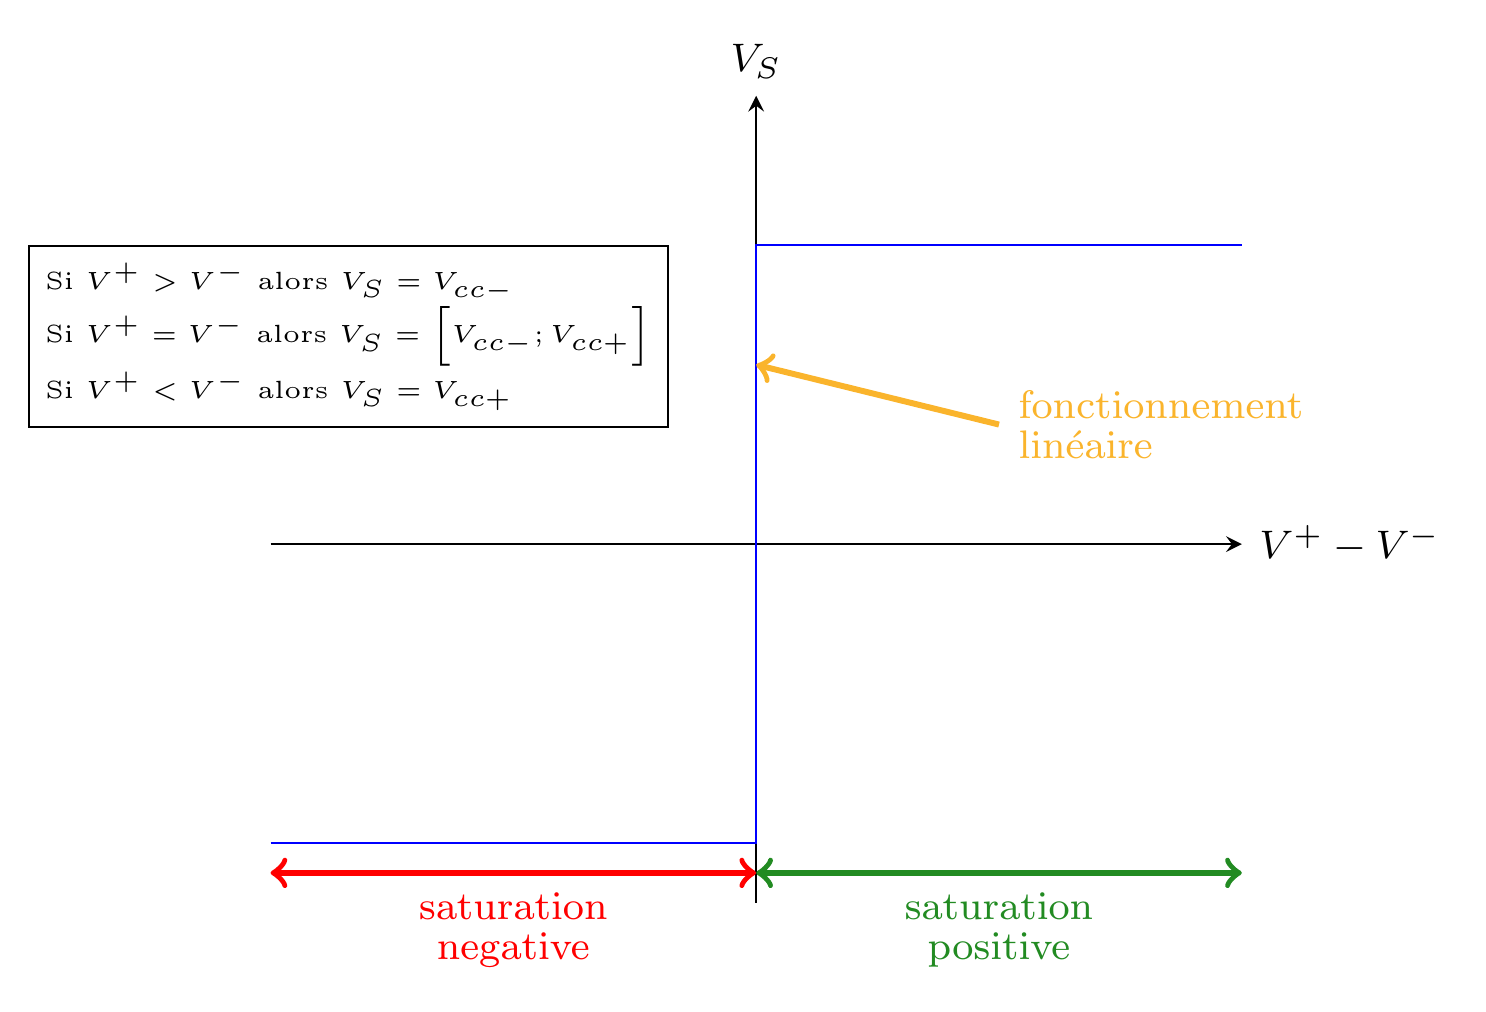
\begin{tikzpicture}[scale=1.8]
        \tikzstyle{every node}=[font=\fontsize{8}{8}\selectfont]
        \begin{axis}[
            axis y line=center,
            axis x line=middle, 
            ticks=none,
            xmin = -1,
            xmax = 1,
            ymin = -1.2,
            ymax = 1.5, 
            ylabel = \(V_S\),
            xlabel = \(V^+-V^-\),
            every axis x label/.style={
                at={(ticklabel* cs:1)},
                anchor=west,
            },
            every axis y label/.style={
                at={(ticklabel* cs:1)},
                anchor=south,
            },
            clip=false,
        ]
        \addplot+[mark=none,] coordinates
        {(-1,-1) (0,-1) (0,1) (1,1)};
        \node[draw,align=left, anchor=north west] at (axis cs:-1.5,1) {\fontsize{5}{5}\selectfont Si \(V^+>V^-\) alors \(V_S=V_{cc-}\)\\\fontsize{5}{5}\selectfont Si \(V^+=V^-\) alors \(V_S=\left[V_{cc-};V_{cc+}\right]\)\\\fontsize{5}{5}\selectfont Si \(V^+<V^-\) alors \(V_S=V_{cc+}\)};
        \draw[<->, very thick, red] (axis cs:-1,-1.1) -- (axis cs:0,-1.1) node[below,pos=0.5,align=center] {saturation\\negative};
        \draw[<-, very thick, Dandelion] (axis cs:0,0.6) -- (axis cs:0.5,0.4) node[right,pos=1,align=left] {fonctionnement\\linéaire};
        \draw[<->, very thick, ForestGreen] (axis cs:0,-1.1) -- (axis cs:1,-1.1) node[below,pos=0.5,align=center] {saturation\\positive};
        \end{axis}
    \end{tikzpicture}
    }
    \caption{Cas d’un ampli op alimenté symétriquement}
    \label{fig:aop-ideal}
\end{figure}

\section{Contre-réaction}

Un amplificateur opérationnel ne s’utilise jamais en \textbf{boucle ouverte}. Il 
est toujours utilisé avec des composants reliant la sortie à l’entrée, un 
principe appelé \textbf{contre-réaction}. Cette contre-réaction permet de 
stabiliser le fonctionnement de l’amplificateur et d’adapter ses performances 
aux besoins du circuit.

On distingue trois types de contre-réaction :

\begin{itemize}
    \item \textbf{Contre-réaction positive} : elle amplifie les variations du signal d’entrée et peut conduire à une saturation rapide du circuit. Elle est utilisée dans des applications comme les comparateurs et les oscillateurs.
    \item \textbf{Contre-réaction négative} : elle réduit l’écart entre l’entrée et la sortie, stabilisant ainsi le fonctionnement de l’amplificateur. Ce type de contre-réaction est largement utilisé dans les circuits d’amplification linéaire.
    \item \textbf{Contre-réaction bilatérale} : elle combine des aspects des deux contre-réactions précédentes et est utilisée dans certains circuits spécifiques nécessitant un contrôle précis du gain et de la réponse en fréquence.
\end{itemize}

\begin{figure}[H]
    \begin{subfigure}[h]{0.49\textwidth}
        \centering
        \includegraphics[width=0.9\textwidth]{opamp-open}
        \caption{Boucle ouverte}
        \label{fig:opamp-open}
    \end{subfigure}
    \begin{subfigure}[h]{0.49\textwidth}
        \centering
        \includegraphics[width=0.9\textwidth]{opamp-CRP}
        \caption{Contre réaction positive}
        \label{fig:opamp-CRP}
    \end{subfigure}
    \vfill
    \begin{subfigure}[h]{0.49\textwidth}
        \centering
        \includegraphics[width=0.9\textwidth]{opamp-CRN}
        \caption{Contre réaction négative}
        \label{fig:opamp-CRN}
    \end{subfigure}
    \begin{subfigure}[h]{0.49\textwidth}
        \centering
        \includegraphics[width=0.9\textwidth]{opamp-CRB}
        \caption{Contre réaction bilatérale}
        \label{fig:opamp-CRB}
    \end{subfigure}
    \caption{Contre-réaction des amplificateurs opérationnels}
    \label{fig:opamp-CR}
\end{figure}

Ici \(\mathsf{Z}\) est un composant ou un ensemble de composants quelconques 
(résistances, condensateurs, etc.).

\begin{itemize}
    \item \textbf{Boucle ouverte} : jamais utilisée en pratique.
    \item \textbf{Contre-réaction positive} : r\'egime satur\'e.
    \item \textbf{Contre-réaction négative} : r\'egime lin\'eaire.
    \item \textbf{Contre-réaction bilatérale} : r\'egime lin\'eaire ou satur\'e.
\end{itemize}

Comme la zone de linéarité d’un amplificateur opérationnel est très réduite, une 
\textbf{contre-réaction négative} est nécessaire pour le maintenir en régime 
linéaire.

\subsection{Effet de la contre-réaction négative}

Lorsque l’on applique une contre-réaction négative :
\begin{itemize}
    \item Si \( V_+ > V_- \), la tension de sortie \( V_S \) augmente. En raison de la contre-réaction négative, \( V_- \) augmente également jusqu’à ce que l’égalité \( V_+ = V_- \) soit atteinte.
    \item Si \( V_+ < V_- \), la tension de sortie \( V_S \) diminue. La contre-réaction négative entraîne alors une diminution de \( V_- \) jusqu’à ce que l’égalité \( V_+ = V_- \) soit rétablie.
    \item Cet ajustement se fait de manière progressive.
    \item Grâce à cette contre-réaction négative, l’amplificateur opérationnel \textbf{converge vers un point d’équilibre} pour sa tension de sortie.
\end{itemize}

\subsection{Effet de la contre-réaction positive}

À l’inverse, lorsque l’on applique une \textbf{contre-réaction positive}, le 
régime saturé est inévitable :

\begin{itemize}
    \item Si \( V_+ > V_- \), la tension de sortie \( V_S \) augmente, ce qui entraîne une augmentation de \( V_+ \) due à la contre-réaction positive, jusqu’à ce que \( V_S \) atteigne \( V_{CC+} \).
    \item Si \( V_+ < V_- \), la tension de sortie \( V_S \) diminue, ce qui provoque une diminution de \( V_+ \) jusqu’à ce que \( V_S \) atteigne \( V_{CC-} \).
    \item Cet ajustement se fait de manière progressive.
    \item Avec une contre-réaction positive, l’amplificateur opérationnel \textbf{diverge systématiquement} vers \( V_{CC+} \) ou \( V_{CC-} \), ce qui le maintient en saturation.
\end{itemize}

\section{Utilités pour l’instrumentation}

Les amplificateurs opérationnels jouent un rôle essentiel dans l’instrumentation 
en permettant le traitement et l’adaptation des signaux issus de divers capteurs.

\subsection{Amplification de signaux}

De nombreux capteurs, tels que les \textbf{thermocouples}, 
\textbf{jauges de contrainte} ou \textbf{photodiodes}, génèrent des tensions ou 
courants très faibles, généralement de l’ordre du \textit{microvolt} (\(\unit{\micro\volt}\)) 
au \textit{millivolt} (\(\unit{\milli\volt}\)). Un amplificateur opérationnel permet d’amplifier ces signaux pour les rendre exploitables par un microcontrôleur ou un système d’acquisition.

\subsection{Adaptation d’impédance}

Certains capteurs possèdent une \textbf{forte impédance de sortie}, ce qui 
signifie qu’ils ne peuvent pas fournir suffisamment de courant pour alimenter un 
circuit suivant. Grâce à son \textbf{impédance d’entrée quasi infinie}, un AOP 
permet de récupérer le signal du capteur sans l’altérer, assurant ainsi un 
transfert d’énergie efficace.

\subsection{Filtrage et réduction du bruit}

Les signaux des capteurs sont souvent affectés par du bruit électrique ou des 
interférences, notamment les perturbations à \SI{50}{Hz} du réseau électrique 
ou les parasites radiofréquence (\textit{RF}). Un AOP peut être utilisé pour 
concevoir des \textbf{filtres actifs}, permettant d’éliminer ces bruits 
parasites avant le traitement du signal.

\subsection{Conversion courant-tension}

Certains capteurs, comme les \textbf{photodiodes} ou les 
\textbf{capteurs électrochimiques}, délivrent un \textbf{courant} plutôt qu’une 
tension. Un AOP configuré en \textbf{convertisseur courant-tension} 
(\( I_{\text{capteur}} \rightarrow V \)) permet de transformer ce signal en une 
tension exploitable par les circuits électroniques.

\subsection{Rejet du mode commun}

Les capteurs à \textbf{ponts résistifs}, tels que les 
\textbf{jauges de contrainte} et les \textbf{capteurs de pression}, nécessitent 
un \textbf{amplificateur différentiel} pour extraire leur signal utile tout en 
éliminant les perturbations en mode commun. Un AOP en configuration 
différentielle permet d’optimiser le rapport signal/bruit dans ces applications.

\subsection{Conditionnement avant numérisation}

Les microcontrôleurs et cartes d’acquisition ne supportent généralement que des 
plages de tensions spécifiques (par exemple, \( 0 - \SI{3.3}{\volt} \) ou 
\( 0 - \SI{5}{\volt} \)). Un AOP permet de :
\begin{itemize}
    \item \textbf{Ajuster} la plage de tension du capteur afin qu’elle corresponde à celle de l’ADC (\textit{Analog-to-Digital Converter}).
    \item \textbf{Décaler (offset)} un signal pour éviter les tensions négatives et le rendre compatible avec l’électronique numérique.
\end{itemize}

\subsection{Compensation des erreurs et linéarisation}

Certains capteurs présentent des \textbf{non-linéarités} ou des erreurs liées à des \textbf{variations de température}. Un AOP peut être utilisé dans un circuit de compensation pour corriger ces erreurs et améliorer la précision des mesures.

\subsection{Conclusion}

Les amplificateurs opérationnels sont indispensables en instrumentation. Sans eux, de nombreux capteurs seraient inexploitables directement, rendant difficile le traitement et l’analyse des signaux dans les systèmes électroniques modernes.
